%--------------------------------------------------------------------------
% Dokumentenklasse
%--------------------------------------------------------------------------

% disable Warning for remreset Package
% \RequirePackage{silence}
% \WarningFilter{remreset}{The remreset package}

\documentclass[
	pagesize,
	fontsize=12pt,
	paper=a4,
	oneside,
   reqno
]{scrartcl}

%--------------------------------------------------------------------------
% Standardpakete 
%--------------------------------------------------------------------------
\usepackage[ngerman]{babel}               % Deutsch Silbentrennung
\usepackage[T1]{fontenc}                  % Font Type
\usepackage[utf8]{inputenc}               % Font Encoding
\usepackage{lmodern}                      % Latin Modern Font
\usepackage{csquotes}                     % Setzen von Zitaten
\usepackage{xspace}                       % setzten von Leerzeichen nach Abkürzungen
\usepackage{microtype}                    % für glattere Seitenränder
\renewcommand*\familydefault{\sfdefault}  % Serifen lose Schrift
%\renewcommand*\familydefault{\ttdefault} % Schreibmaschinenschrift

%--------------------------------------------------------------------------
% Extra Packages
%--------------------------------------------------------------------------

% Abkürzungspaket
\usepackage{acronym}

% Symbolverzeichnis
\usepackage[symbols,nogroupskip,nonumberlist,sort=use]{glossaries-extra}

% \makenoidxglossaries

\glsxtrnewsymbol[description={Gewichtskraft}]{FG}{\ensuremath{F_{\mathrm{G}}}}
\glsxtrnewsymbol[description={Gewichtskraft in Bewegungsrichtung}]{FG1}{\ensuremath{F^{'}_{\mathrm{G}}}}
\glsxtrnewsymbol[description={Bewegungskraft des Schlittens}]{Fa}{\ensuremath{F_{\mathrm{a}}}}
\glsxtrnewsymbol[description={Pendelkraft}]{FP}{\ensuremath{F_{\mathrm{P}}}}
\glsxtrnewsymbol[description={Pendelkraft in Bewegungsrichtung}]{FP1}{\ensuremath{F^{'}_{\mathrm{P}}}}
\glsxtrnewsymbol[description={Reibkraft}]{Ff}{\ensuremath{F_{\mathrm{f}}}}
\glsxtrnewsymbol[description={Coulombsche Reibung}]{FC}{\ensuremath{F_{\mathrm{C}}}}
\glsxtrnewsymbol[description={Gesamtkraft}]{Fges}{\ensuremath{F_{\mathrm{ges}}}}
\glsxtrnewsymbol[description={Pendelmoment}]{MP}{\ensuremath{M_{\mathrm{P}}}}
\glsxtrnewsymbol[description={Gewichtsmoment}]{MG}{\ensuremath{M_{\mathrm{G}}}}
\glsxtrnewsymbol[description={Reibmoment}]{Mf}{\ensuremath{M_{\mathrm{f}}}}
\glsxtrnewsymbol[description={Gesamtmoment}]{Mges}{\ensuremath{M_{\mathrm{ges}}}}

% Mathe Pakete
\usepackage{amsmath}
\DeclareMathOperator{\sgn}{sgn}
\usepackage{thmtools}
\usepackage{amsfonts}
\usepackage{amssymb}
\usepackage{mathtools}
\usepackage{breqn}

% Listenumgebungen
\usepackage{listings}
\usepackage{paralist}
\usepackage{enumitem}
\usepackage{adjustbox}

% Demo Text
\usepackage{blindtext}

% Farb-Pakete
\usepackage{xcolor}
\usepackage{fancyvrb}
\usepackage{colortbl}

% Farbedefinitionen
\definecolor{htw}{RGB}{120, 184, 2}
\definecolor{ccW}{RGB}{255,255,255}
\definecolor{ccR}{RGB}{197,14,31}
\definecolor{ccG}{RGB}{113,113,113}
\definecolor{ccL}{RGB}{220,220,220}
\definecolor{ccS}{RGB}{0,0,0}
\definecolor{ccB}{RGB}{68,73,159}
\definecolor{ccD}{RGB}{0,0,80}
\definecolor{grey}{RGB}{200,200,200}
\definecolor{lightGrey}{RGB}{230,230,230}

% Für erweiterte Tabellen
\usepackage{longtable}
\usepackage{tabularx}
\usepackage{float}
\usepackage{multirow}
\usepackage{makecell}
% \setlength{\tabcolsep}{0.5em}       % for the horizontal padding
% {\renewcommand{\arraystretch}{1.8}  % for the vertical padding
% \usepackage{ragged2e}
% \newcolumntype{R}[1]{>{\RaggedRight}p{#1}}

% Einheitenpaket
\usepackage[exponent-product = \cdot]{siunitx}
\sisetup{locale=DE}
\sisetup{parse-numbers = false}

\makeatletter
\renewcommand\@dotsep{5}
\makeatother

% Pakete für Grafiken
\usepackage{graphicx}
\usepackage{wrapfig}
\usepackage{overpic}
\usepackage{epstopdf}
\usepackage{caption}
\usepackage{subcaption}
\usepackage{rotating}
\usepackage{lscape}
% \captionsetup[subfigure]{list=true, font=normalsize, labelformat=brace, position=top} %setup für subfigure captions

% Diagramm-/Grafikerstellung
\usepackage{pstricks}
\usepackage{tikz}
\makeatletter
\pgfkeys{/pgf/.cd,
  parallelepiped offset x/.initial=2mm,
  parallelepiped offset y/.initial=2mm
}
\pgfdeclareshape{parallelepiped}
{
  \inheritsavedanchors[from=rectangle] % this is nearly a rectangle
  \inheritanchorborder[from=rectangle]
  \inheritanchor[from=rectangle]{north}
  \inheritanchor[from=rectangle]{north west}
  \inheritanchor[from=rectangle]{north east}
  \inheritanchor[from=rectangle]{center}
  \inheritanchor[from=rectangle]{west}
  \inheritanchor[from=rectangle]{east}
  \inheritanchor[from=rectangle]{mid}
  \inheritanchor[from=rectangle]{mid west}
  \inheritanchor[from=rectangle]{mid east}
  \inheritanchor[from=rectangle]{base}
  \inheritanchor[from=rectangle]{base west}
  \inheritanchor[from=rectangle]{base east}
  \inheritanchor[from=rectangle]{south}
  \inheritanchor[from=rectangle]{south west}
  \inheritanchor[from=rectangle]{south east}
  \backgroundpath{
    % store lower right in xa/ya and upper right in xb/yb
    \southwest \pgf@xa=\pgf@x \pgf@ya=\pgf@y
    \northeast \pgf@xb=\pgf@x \pgf@yb=\pgf@y
    \pgfmathsetlength\pgfutil@tempdima{\pgfkeysvalueof{/pgf/parallelepiped offset x}}
    \pgfmathsetlength\pgfutil@tempdimb{\pgfkeysvalueof{/pgf/parallelepiped offset y}}
    \def\ppd@offset{\pgfpoint{\pgfutil@tempdima}{\pgfutil@tempdimb}}
    \pgfpathmoveto{\pgfqpoint{\pgf@xa}{\pgf@ya}}
    \pgfpathlineto{\pgfqpoint{\pgf@xb}{\pgf@ya}}
    \pgfpathlineto{\pgfqpoint{\pgf@xb}{\pgf@yb}}
    \pgfpathlineto{\pgfqpoint{\pgf@xa}{\pgf@yb}}
    \pgfpathclose
    \pgfpathmoveto{\pgfqpoint{\pgf@xb}{\pgf@ya}}
    \pgfpathlineto{\pgfpointadd{\pgfpoint{\pgf@xb}{\pgf@ya}}{\ppd@offset}}
    \pgfpathlineto{\pgfpointadd{\pgfpoint{\pgf@xb}{\pgf@yb}}{\ppd@offset}}
    \pgfpathlineto{\pgfpointadd{\pgfpoint{\pgf@xa}{\pgf@yb}}{\ppd@offset}}
    \pgfpathlineto{\pgfqpoint{\pgf@xa}{\pgf@yb}}
    \pgfpathmoveto{\pgfqpoint{\pgf@xb}{\pgf@yb}}
    \pgfpathlineto{\pgfpointadd{\pgfpoint{\pgf@xb}{\pgf@yb}}{\ppd@offset}}
  }
}
\makeatother
\usetikzlibrary{math}
\usepackage{pgfplots}
\pgfplotsset{compat=1.5}
\usetikzlibrary{intersections,positioning,arrows,automata,calc,patterns,shapes.multipart,fit,backgrounds,decorations.pathreplacing}
\usetikzlibrary{decorations,shapes.geometric}
\usetikzlibrary{matrix,calc,angles,positioning,quotes}
% \usepackage{tikz-uml}

\usepackage{pgfkeys}
\usepackage{pgfopts}
\usepackage{ifthen}
\usepackage{xstring}
\usepackage{calc}
\usepackage{pst-plot,pst-bar,pst-node} % Balkendiagramme
\usepackage{capt-of}
\usepackage{incgraph} % Fullscreen Images
\usepackage{pdfpages} % Include external pdf pages

\usepackage{latexsym}
\usepackage{censor}
\usepackage{here}
% \StopCensoring        % Auskommentiert wird der Text entschwaerzt 
% \censor{Oszilloskop}  % Befehl zum einschwärzen
\usepackage{trfsigns}   % Transformation Symbol o---o \laplace and \Laplace
\usepackage{circuitikz}

\usepackage{multido}

% Verlinkungen im Text
\usepackage{url}
\usepackage{hyperref}
\PassOptionsToPackage{hyphens}{url}
\hypersetup{hidelinks}
\urlstyle{same}

%--------------------------------------------------------------------------
% Eigene Befehle
%--------------------------------------------------------------------------
% Test 
% \renewcommand{\thesection}{\arabic{section}} % Section startet mit 1.0 und nicht mit 0.1

%------------sectioning command-------------------
% The sectioning command one level down the hierarchy from \subsubsection is called \paragraph followed by \subparagraph
% to include this in your table of contents

% for paragraph
\setcounter{tocdepth}{4}
\setcounter{secnumdepth}{4}
% for subparagraph
\setcounter{tocdepth}{5}
\setcounter{secnumdepth}{5}

% Abkürzungen durch Kommandos setzen
\newcommand{\bspw}{bspw.\xspace}
\newcommand{\bzw}{bzw.\xspace}
\newcommand{\etc}{etc.\xspace}
\newcommand{\zB}{z.\,B.\xspace}
\newcommand{\EV}{e.\,V.\xspace}
\newcommand{\zT}{z.\,T.\xspace}
\newcommand{\iVm}{i.\,V.\,m.\xspace}
\newcommand{\idR}{i.\,d.\,R.\xspace}
\newcommand{\ihv}{i.\,H.\,v.\xspace}
\newcommand{\ua}{u.\,a.\xspace}
\newcommand{\dH}{d.\,h.\xspace}
\newcommand{\vgl}{vgl.\xspace}
\newcommand{\ca}{ca.\xspace}
\newcommand{\dV}{d.\,Verf.}
\newcommand{\RNr}{Rn.\xspace}
\newcommand{\oa}{o.\,{ä}.\xspace}
\newcommand{\vC}{v.\,Chr.\xspace}
\newcommand{\nC}{n.\,Chr.\xspace}
\newcommand{\vA}{v.\,a.\xspace}
\newcommand{\eng}{engl.\xspace}
\newcommand{\tabitem}{~~\llap{\textbullet}~~}

%------------Zitate-------------------------------
\newcommand*{\zitat}[2]{%
   \normalfont\small
   \begin{quote}
   \glqq#1\grqq \par
   #2
   \end{quote}
   \normalsize
}
\newcommand*{\zitatmitueberschrift}[3]{%
   \normalfont\small
   \begin{quote} #3
   \glqq#1\grqq \par
   #2
   \end{quote}
   \normalsize
}
\newcommand*{\zitext}[2]{%
   \glqq#1\grqq\ %
   [#2]%
}

%-----------Seitendesign--------------------------
\usepackage[width=15.5cm, height=23cm, includeheadfoot]{geometry}
\geometry{paper=a4paper}
% \usepackage[left=6cm,right=1cm,top=1.5cm, bottom=1cm, includeheadfoot]{geometry}
% \newgeometry{oneside}
% \setlength{\voffset}{0cm}
\setlength{\headheight}{1.1\baselineskip} % increase headheight
\setlength{\footheight}{28.99998pt}       % increase foodheight
\setlength{\parindent}{0cm}               % Einrücken nach \newline
\setlength{\footskip}{86pt}               % Move Footer down
% \setlength{\topmargin}{0cm}
% \setlength{\marginparsep}{0.5cm}
% \setlength{\marginparwidth}{1.5cm}
% \setlength{\textwidth}{16cm}
% \setlength{\textheight}{23cm}
% \setlength{\oddsidemargin}{1cm}
% \setlength{\evensidemargin}{2cm}

%----------Kopf & Fußzeile------------------------
% \usepackage[headsepline,footsepline]{scrpage2}
\usepackage[headsepline]{scrlayer-scrpage}
\pagestyle{scrheadings}
\clearpairofpagestyles
\ihead{\headmark}
\automark{section}
\chead{}
\ohead{
\includegraphics[scale=0.09]{Bilder/HTWLogoKopfzeile.png} \nocite{HTWklein}}
\ifoot{Sebastian Richter\\ Aaron Zielstorff}
\cfoot{\pagemark}
\ofoot{VA1 Moderne Methoden\\ der Regelungstechnik}

%--------------------------------------------------------------------------
% Beginn des Dokuments
%--------------------------------------------------------------------------
\begin{document}

%----------Deckblatt----------------------------- 
\begin{titlepage}
   \pagestyle{empty} % setzt Pagestyle-Befehl

   % HTW Logo
   \begin{flushright}
   
\includegraphics[scale=.07]{Bilder/LogoHTWBerlin.png}  \nocite{HTWgross}
   \end{flushright}

   \vspace{1cm}

   % Titel
   \begin{center}
      \Huge{\textbf{Buck Converter: Moderne Methoden der Regelungstechnik (VA1)}} \\
   \end{center}

   \vspace{3cm}

   % Name
   \begin{flushleft}
      \begin{tabular}{l c l }
         \textbf{Name: }&\hspace{1 cm} &\textbf{Matrikelnummer:} \\
         Sebastian Richter  & & 572906 \\
         Aaron Zielstorff   & & 567183 \\
      \end{tabular}
   \end{flushleft}

   \vspace{1cm}

   % Daten
   \begin{tabular}{l l}
      \textbf{Fachbereich:}   & FB1                                                 \\
      \textbf{Studiengang:}   & M.\xspace Elektrotechnik                            \\
      \textbf{Fachsemester:}  & 2.\xspace FS                                        \\
      \textbf{Fach:}          & VA1 Moderne Methoden der Regelungstechnik           \\
      \textbf{Dozent:}        & Prof.\xspace Dr.\xspace -Ing.\xspace Horst Schulte  \\
      \textbf{Abgabe am:}     & 25.\xspace Juli 2022                                \\ 
   \end{tabular}
\end{titlepage}
\clearpage

%--------Inhaltsverzeichnis-----------------------
\renewcommand{\contentsname}{Inhaltsverzeichnis}
\tableofcontents
\clearpage

%--------Abbildungsverzeichnis--------------------
\renewcommand{\listfigurename}{Abbildungsverzeichnis}
\renewcommand*{\figurename}{Abb.}
\listoffigures
% \clearpage

%--------Tabellenverzeichnis----------------------
\renewcommand*{\listtablename}{Tabellenverzeichnis}
\renewcommand*{\tablename}{Tab.}
\listoftables
\clearpage

%----------Symbolverzeichnis----------------------
% \printnoidxglossary[type=symbols,style=long,title={Symbolverzeichnis}]
% \clearpage

%---------Kapitel/Text----------------------------

\section{Einführung in die Regelaufgabe} \label{sec:Einfuehrung}

Photovoltaikanlagen enthalten viele Tausend einzelne Photovoltaikzellen. Jede Einzelne wandelt einfallende Sonnenstrahlung (direkt und indirekt) in elektrischen Strom um. Unter Vernachlässigung von Verlusten in Kabeln, Wandlerverlusten und Leistungsfehlanpassungen ist die erzeugte Leistung von PV-Systemen, die Anzahl aller enthaltenen Zellen multipliziert mit der Leistung einer einzelnen Zelle. Über diese Annahme ist es möglich, das mathematische Modell der gesamten PV-Anlage für die Systemanalyse abzuleiten. \\
Die Grundeinheiten einer PV-Anlage sind die PV-Module oder auch Solarzellen. Ein Standard-PV-Modul besteht aus 48 bis 73 in Reihe geschalteten Zellen, die in einen Rahmen montiert sind. PV-Anlagen werden in der Regel durch Reihen- und Parallelschaltungen von Modulen zusammengesetzt. Solarmodule werden in Reihe geschaltet (sog.\xspace \glqq Strings\grqq{}), um die Ausgangsspannung zu erhöhen. Parallel geschaltete Strings bilden ein \glqq Array\grqq{}, in dem die Leistungskapazität von Tausenden bis Millionen Watt aufgebaut werden kann. \\
Das mathematische Modell des PV-Generators ergibt sich aus der Zusammenfassung aller PV-Module, die durch das Modell einer einzelnen Zelle beschrieben werden. Strom und Spannung werden in geeigneter Weise multipliziert. Dazu wird die Einzelzelle durch ein Ersatzschaltbild modelliert, das aus einer einstrahlungsabhängigen Stromquelle, einem Modell der Diode $D$ und Shunt-Widerstand $R_{\mathrm{h}}$ besteht, wie in \autoref{fig:Bild1} (links) dargestellt. Die Einstrahlung $S$ mit der physikalischen Einheit $\SI{}{\frac{W}{m^2}}$ bezieht sich auf die direkte (normal zum PV-Zellenfeld) und die indirekte Einstrahlung. \\
\newline
Um die Spannung von PV-Anlagen zu regeln, werden Gleichspannungswandler eingesetzt. Die Ausgangsspannung des Wandlers kann eingestellt werden und unterscheidet sich von der Eingangsspannung. Eine grundlegende Gleichspannungswandlerschaltung ist der so genannte Buck Converter (Tiefsetzsteller), welcher ebenfalls in \autoref{fig:Bild1} (rechts) dargestellt ist. \\
Die Pulsweitenmodulation (PWM) ermöglicht die Steuerung und Regelung der gesamten Ausgangsspannung. Die PWM stellt ein Rechtecksignal bereit, welches zwischen 0 und 1 schaltet. Typische Schaltfrequenzen liegen zwischen $f_{\mathrm{SW}} = \SI{1}{kHz} \ldots \SI{1}{MHz}$. Im Falle der konkreten Anlage beträgt die Schaltfrequenz $f_{\mathrm{SW}} = \SI{5}{kHz}$. In der Praxis werden \zB MOSFET's als Schalter eingesetzt. Die Ausgangsspannung hinter dem MOSFET (siehe ebenfalls \autoref{fig:Bild1} (mittig)) wechselt somit zwischen Null und der Ausgangsspannung des Wandlers $v_{\mathrm{DC}}$. Das Tastverhältnis (Duty Cycle) $d$ beschreibt die Zeitverhältnisse des Rechtecksignals, also wann der Schalter (MOSFET) in Position 0 \bzw 1 ist. Der Duty Cycle lässt sich wie folgt berechnen:

\begin{align}
    d = \frac{v_{\mathrm{DC}}}{v_{\mathrm{PV}}} \quad \text{\bzw} \quad d = \frac{i_{\mathrm{PV}}}{i_{\mathrm{DC}}}
    \label{eq:Gleichung1}
\end{align}

Nachfolgend befindet sich die Darstellung der Modellparameter/Konstanten zur Modellierung des Buck Converters (siehe \autoref{tab:Tabelle1}).

\begin{table}[H]
    \centering
    \begin{tabular}{|lll|}
        \hline
        \rowcolor{grey}
        \textbf{Symbol}          & \textbf{Parameter}                               & \textbf{Wert}                            \\ \hline
        \rowcolor{lightGrey}
        \multicolumn{3}{|c|}{Standard Testbedingungen (STC)}                                                                   \\ \hline
        $T_{\mathrm{c,STC}}$     & PV Zelltemperatur bei STC                        & $\SI{298}{K}$                            \\
        $S_{\mathrm{STC}}$       & Bestrahlung bei STC                              & $\SI{1000}{\frac{W}{m^2}}$               \\
        $v_{\mathrm{T,STC}}$     & Thermische Spannung der p-n Sperrschicht bei STC & $\SI{25.7 \cdot 10^{-3}}{V}$             \\
        $i_{\mathrm{ph,sc,STC}}$ & Kurzschlussstrom des Diodenmodells bei STC       & $\SI{9.272}{A}$                          \\
        $v_{\mathrm{oc,STC}}$    & Leerlaufspannung bei STC                         & $\SI{0.644}{V}$                          \\ \hline
        \rowcolor{lightGrey}
        \multicolumn{3}{|c|}{Maximaler Leistungspunkt (MPP)}                                                                   \\ \hline
        $i_{\mathrm{PV,MPP}}$    & Gesamtstrom des PV Parks beim MPP                & $\SI{2902.13}{A}$                        \\
        $v_{\mathrm{PV,MPP}}$    & Gesamtspannung des PV Parks beim MPP             & $\SI{1049.13}{V}$                        \\
        $P_{\mathrm{MPP}}$       & Gesamtleistung des PV Parks beim MPP             & $\SI{30447.11}{W}$                       \\ \hline
        \rowcolor{lightGrey}
        \multicolumn{3}{|c|}{Weitere Parameter}                                                                                \\ \hline
        $R_{\mathrm{h}}$         & Shunt-Widerstand im Einzeldiodenmodell           & $\SI{10.196}{\Omega}$                    \\
        $v_{\mathrm{DC}}$        & Ausgangsgleichspannung                           & $\SI{900}{V}$                            \\
        $N_{\mathrm{cell,p}}$    & Anzahl paralleler Zellen pro Modul               & 1                                        \\
        $N_{\mathrm{cell,s}}$    & Anzahl serieller Zellen pro Modul                & 72                                       \\
        $N_{\mathrm{mod,p}}$     & Anzahl paralleler Module pro Anlage              & 336                                      \\
        $N_{\mathrm{mod,s}}$     & Anzahl serieller Module pro Anlage               & 27                                       \\
        $N_{\mathrm{p}}$         & Anzahl paralleler Zellen pro Anlage              & $\SI{336}{}$                             \\
        $N_{\mathrm{s}}$         & Anzahl serieller Zellen pro Anlage               & $\SI{1944}{}$                            \\
        $k$                      & Boltzmann Konstante                              & $\SI{1.381 \cdot 10^{-23}}{\frac{J}{K}}$ \\
        $q$                      & Elementarladung                                  & $\SI{1.602 \cdot 10^{-19}}{C}$           \\
        $A_{\mathrm{n}}$         & Dioden-Idealitätsfaktor im Einzeldiodenmodell    & $\SI{1.374}{}$                           \\
        $\alpha _{\mathrm{T}}$   & Temperaturkoeffizient des PV-Stroms              & $\SI{0.06 \cdot 10^{-2}}{}$              \\
        $\beta _{\mathrm{T}}$    & Temperaturkoeffizient der PV-Spannung            & $\SI{-0.36 \cdot 10^{-2}}{}$             \\ \hline
    \end{tabular}
    \caption{Modellparameter des Buck Converters}
    \label{tab:Tabelle1}
\end{table}

Ziel der Regelung soll es sein, die Ausgangsspannung $v_{\mathrm{DC}}$ konstant bei $\SI{900}{V}$ zu halten. Die einzelnen PV-Zellen wurden im Vorhinein für verschiedene Bestrahlungen und Temperaturen messtechnisch analysiert. Die nachfolgende Modellierung erfolgt zunächst für eine konstante Bestrahlung mit $S = \SI{1000}{\frac{W}{m^2}}$ bei einer konstanten Zelltemperatur von $T_{\mathrm{c}} = \SI{298}{K}$.

\begin{figure}[H]
   \centering
   \fbox{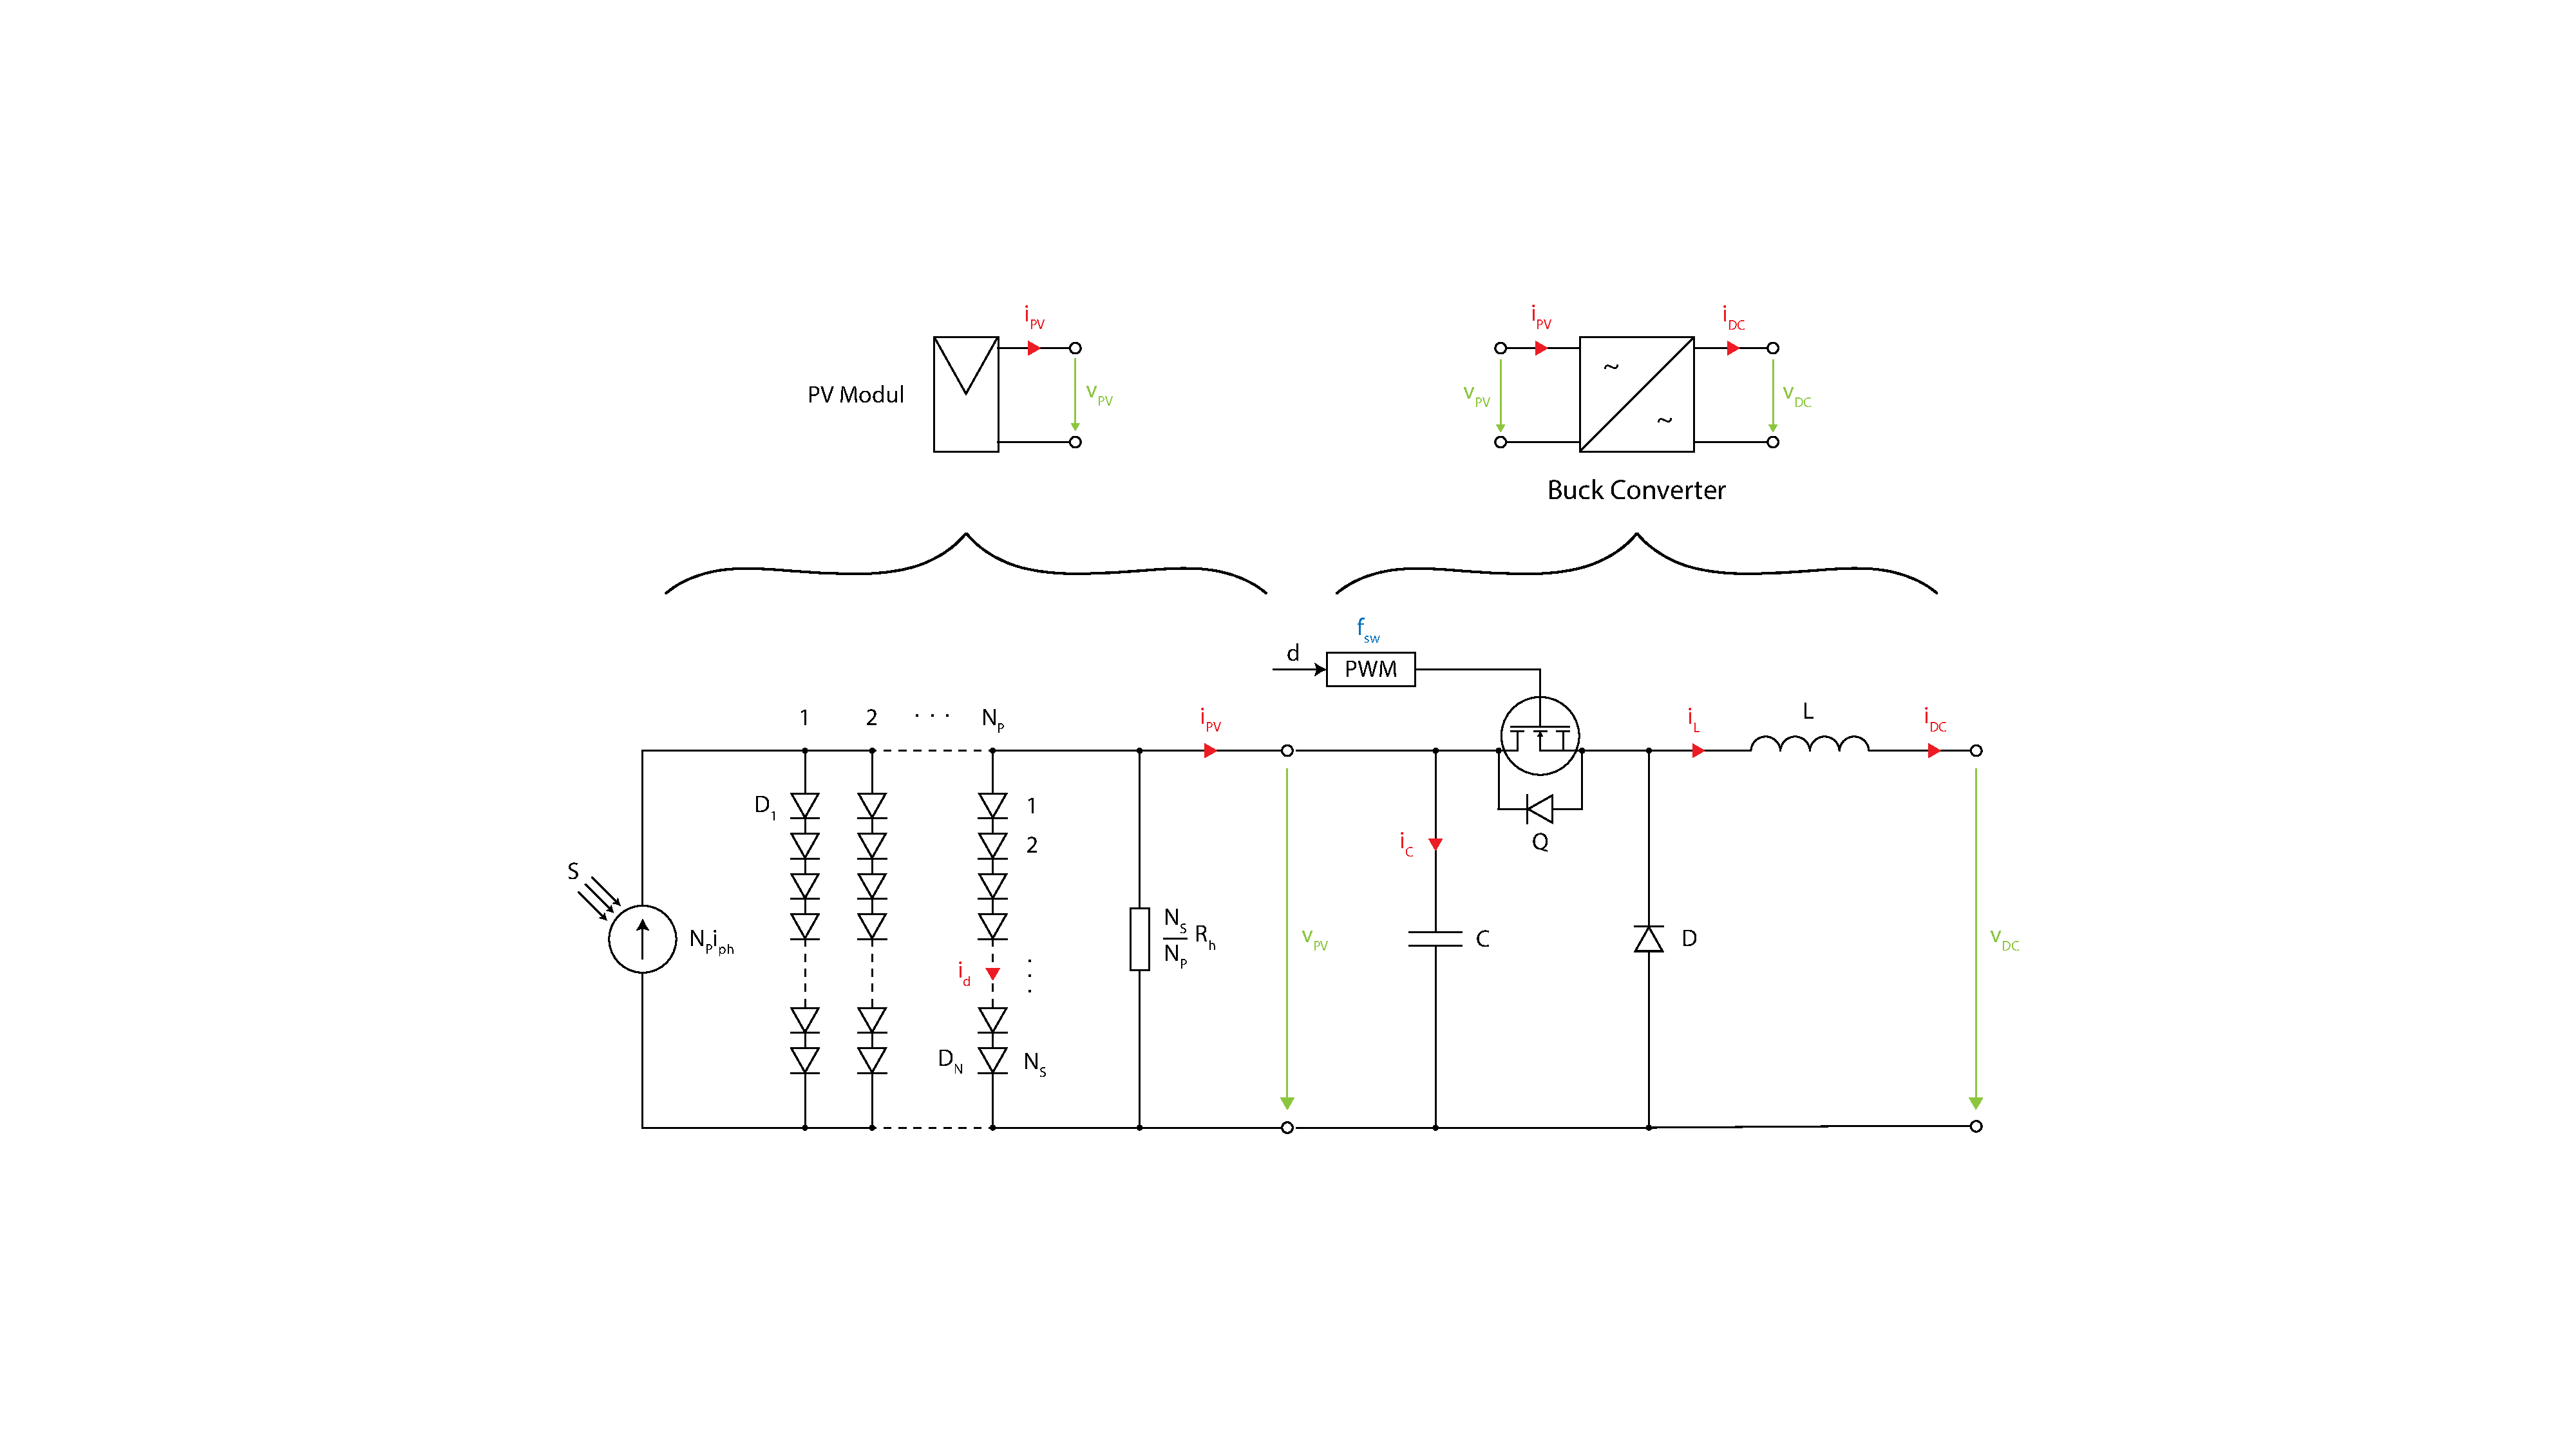
\includegraphics[width=1.0\textwidth]{Bilder/Buck_Zeichnung.pdf}}
   \caption[Skizze der Regelaufgabe]{Übersichtsschaltbild des Buck Converters als zu regelndes System inklusive Photovoltaik Anlage}
   \label{fig:Bild1}
\end{figure}

\section{Modellierung: Energiemethode nach Lagrange}

\subsection{Ansatz}

Die nachfolgende Gleichung zeigt den Lagrange Ansatz unter Berücksichtigung der dissipativen Funktion. Diese besagt in Erweiterung zu der Lagrange-Formulierung, dass Energie in einem Vorgang in Wärme umgewandelt wird. Mit Hilfe der dissipativen Funktion können Reibungsverluste bei der Energiemethode nach Lagrange berücksichtigt werden.

\begin{align} \label{eq:Gleichung1}
    \frac{d}{dt} \left(\frac{\partial L}{\partial \dot{q_{\mathrm{i}}}}\right) - \frac{\partial L}{\partial q_{\mathrm{i}}} + \frac{\partial D}{\partial \dot{q_{\mathrm{i}}}} = F_{\mathrm{i}}
\end{align}

\subsection{Freiheitsgrade und Zwangsbedingungen}

In \autoref{fig:Bild1} sind zwei Massepunkte im $\mathbb{R}^2$ zu erkennen. Somit gilt grundsätzlich:
\begin{itemize}
    \item 2 Punkte: 4 Freiheitsgrade (FHG)
\end{itemize}

Das inverse Pendel besitzt jedoch auch zwei Zwangsbedingungen, die wie folgt formuliert werden können:

\begin{itemize}
    \item Der Wagen kann sich nur horizontal bewegen: \\ $y_{\mathrm{M}} = 0$
    \item Die Masse $m$ am Ende des Pendels ist mit dem Wagen gekoppelt: \\ $(y_{\mathrm{M}} - y_{\mathrm{m}})^2 + (x_{\mathrm{M}} - x_{\mathrm{m}})^2 = l^2$
\end{itemize}

Somit bleiben am Ende noch zwei Freiheitsgrade (FHG) übrig.

\subsection{Generalisierte Koordinaten}

Aus den verbliebenen Freiheitsgraden werden die beiden generalisierten Koordinaten abgeleitet.

\begin{itemize}
    \item $q_{\mathrm{1}} = x_{\mathrm{M}}$
    \item $q_{\mathrm{2}} = \varphi$
\end{itemize}

\subsection{Berechnung der kinetischen und potentiellen Energie}

Der Ansatz zur Berechnung einer kinetischen Energie ist nachfolgend gezeigt.

\begin{align}\label{eq:Gleichung2}
    E_{\mathrm{kin}} = \frac{1}{2} \cdot m \cdot v^2
\end{align}

Zu berücksichtigen ist, dass beide Massen ($m$ und $M$) eine kinetische Energie besitzen (\autoref{eq:Gleichung3} und \autoref{eq:Gleichung4}).

\begin{align}
    E_{\mathrm{kin}} &= \frac{1}{2} \cdot M \cdot \dot{x}_{\mathrm{M}}^2 + \frac{1}{2} \cdot m \cdot v_{\mathrm{m}}^2 \label{eq:Gleichung3} \\
    E_{\mathrm{kin}} &= \frac{1}{2} \cdot M \cdot \dot{x}_{\mathrm{M}}^2 + \frac{1}{2} \cdot m \cdot \left(\dot{x}_{\mathrm{m}}^2 + \dot{y}_{\mathrm{m}}^2\right) \label{eq:Gleichung4}
\end{align}

Weiter gilt:

\begin{align*}
    x_{\mathrm{m}} &= x_{\mathrm{M}} + l \cdot \sin({\varphi}) \\
    y_{\mathrm{m}} &= l \cdot \cos({\varphi}) \\
    \dot{x_{\mathrm{m}}} &= \dot{x_{\mathrm{M}}} + l \cdot \dot{\varphi} \cdot \cos{\varphi} \\
    \dot{y_{\mathrm{m}}} &= -l \cdot \dot{\varphi} \cdot \sin({\varphi})
\end{align*}

Daraus resultiert:

\begin{dmath*}
    E_{\mathrm{kin}} = \frac{1}{2} \cdot M \cdot \dot{x}_{\mathrm{M}}^2 + \frac{1}{2} \cdot m \cdot \left(\left(\dot{x}_{\mathrm{M}} + l \cdot \dot{\varphi} \cdot \cos({\varphi})\right)^2 + \left( -l \cdot \dot{\varphi} \cdot \sin({\varphi})\right)^2\right) \\
    = \frac{1}{2} \cdot M \cdot \dot{x}_{\mathrm{M}}^2 + \frac{1}{2} \cdot m \cdot \left(\dot{x}_{\mathrm{M}}^2 + 2 \cdot \dot{x}_{\mathrm{M}} \cdot l \cdot \dot{\varphi} \cdot \cos({\varphi}) + l^2 \cdot \dot{\varphi}^2 \cdot \cos^2(\varphi) + l^2 \cdot \dot{\varphi}^2 \cdot \sin^2(\varphi)\right) \\
    = \frac{1}{2} \cdot M \cdot \dot{x}_{\mathrm{M}}^2 + \frac{1}{2} \cdot m \cdot \dot{x}_{\mathrm{M}}^2 + m \cdot \dot{x}_{\mathrm{M}} \cdot l \cdot \dot{\varphi} \cdot \cos({\varphi}) + \frac{1}{2} \cdot m \cdot l^2 \cdot \dot{\varphi}^2 \cdot \cos^2(\varphi) + \frac{1}{2} \cdot m \cdot l^2 \cdot \dot{\varphi}^2 \cdot \sin^2(\varphi)
\end{dmath*}

Durch das Zusammenfassen der vorangegangenen Beziehung folgt \autoref{eq:Gleichung5} für die gesamte kinetische Energie des Systems.

\begin{align} \label{eq:Gleichung5}
    E_{\mathrm{kin}} = \frac{1}{2} \cdot \dot{x}_{\mathrm{M}}^2 \cdot (M + m) + \frac{1}{2} \cdot m \cdot \left( 2 \cdot \dot{x}_{\mathrm{M}} \cdot l \cdot \dot{\varphi} \cdot \cos({\varphi}) + l^2 \cdot \dot{\varphi}^2\right)
\end{align}

Ausschließlich die Masse $m$ am Pendelende besitzt eine für den Lagrange-Formalismus relevante potentielle Energie (\autoref{eq:Gleichung6}).

\begin{align}
    E_{\mathrm{pot}} &= m \cdot g \cdot h \nonumber \\
    E_{\mathrm{pot}} &= m \cdot g \cdot y_{\mathrm{m}} \nonumber \\
    E_{\mathrm{pot}} &= m \cdot g \cdot l \cdot \cos({\varphi}) \label{eq:Gleichung6}
\end{align}

\subsection{Herleitung der Bewegungsgleichungen}

Die Lagrange-Funktion wird aus der Differenz der kinetischen und der potentiellen Energie berechnet (\autoref{eq:Gleichung7}).

\begin{align} 
        L &= E_{\mathrm{kin}} - E_{\mathrm{pot}}  \label{eq:Gleichung7} \\ 
        L &= \frac{1}{2} \cdot \dot{x}_{\mathrm{M}}^2 \cdot (M + m) + \frac{1}{2} \cdot m \cdot \left( 2 \cdot \dot{x}_{\mathrm{M}} \cdot l \cdot \dot{\varphi} \cdot \cos({\varphi}) + l^2 \cdot \dot{\varphi}^2\right) - m \cdot g \cdot l \cdot \cos({\varphi}) \label{eq:Gleichung8}
\end{align}

Im ersten Schritt wird die Bewegungsgleichung des Wagens hergeleitet. Dafür wird zunächst \autoref{eq:Gleichung8} nach der ersten zeitlichen Ableitung der generalisierten Koordinate $x_{\mathrm{M}}$ partiell differenziert:

\begin{align}\label{eq:Gleichung9}
    \frac{\partial L}{\partial \dot{x}_{\mathrm{M}}} = (M + m) \cdot \dot{x}_{\mathrm{M}} + m \cdot l \cdot \dot{\varphi} \cdot \cos(\varphi)
\end{align}

Die vorangegangene Gleichung wird zeitlich differenziert:

\begin{align}\label{eq:Gleichung10}
    \frac{d}{dt}\left(\frac{\partial L}{\partial \dot{x}_{\mathrm{M}}}\right) = (M + m) \cdot \ddot{x}_{\mathrm{M}} + m \cdot l \cdot \left(\ddot{\varphi} \cdot \cos(\varphi) - \dot{\varphi}^2 \cdot \sin(\varphi) \right)
\end{align}

Im zweiten Schritt wird die Lagrange-Funktion nach der generalisierten Koordinate $x_{\mathrm{M}}$ abgeleitet.

\begin{align}\label{eq:Gleichung11}
    \frac{\partial L}{\partial x_{\mathrm{M}}} = 0
\end{align}

Abschließend wird die dissipative Funktion nach der 1. Ableitung der generalisierten Koordinate $x_{\mathrm{M}}$ differenziert.

\begin{align}\label{eq:Gleichung12}
    \frac{\partial D}{\partial \dot{x_{\mathrm{M}}}} = d \cdot \dot{x_{\mathrm{M}}}
\end{align}

Durch das Einsetzen der \autoref{eq:Gleichung9} bis \autoref{eq:Gleichung12} in den Ansatz aus \autoref{eq:Gleichung1} resultiert die vollständige Bewegungsgleichung des Wagens.

\begin{align}\label{eq:Gleichung13}
    (M + m) \cdot \ddot x_{\mathrm{M}} + m \cdot l \cdot \left( \ddot \varphi \cdot \cos({\varphi}) - \dot \varphi^2 \cdot \sin({\varphi})\right) + d \cdot \dot x_{\mathrm{M}} = F_{\mathrm{a}}
\end{align}

Analog wird die Bewegungsgleichung des Pendels entwickelt. Hierbei wird zunächst \autoref{eq:Gleichung8} nach der 1. Ableitung der generalisierten Koordinate $\varphi$ partiell differenziert.

\begin{align}\label{eq:Gleichung14}
    \frac{\partial L}{\partial \dot{\varphi}} = m \cdot l \cdot \dot{x}_{\mathrm{M}} \cdot \cos(\varphi) + m \cdot l^2 \cdot \dot{\varphi}
\end{align}

Die vorangegangene Gleichung wird nach der Zeit abgeleitet:

\begin{align}\label{eq:Gleichung15}
    \frac{d}{dt}\left(\frac{\partial L}{\partial \dot{\varphi}}\right) = m \cdot l \cdot \left(\ddot{x}_{\mathrm{M}} \cdot  \cos(\varphi) - \dot{x}_{\mathrm{M}} \cdot \sin(\varphi) \cdot \dot{\varphi}\right) + m \cdot l^2 \cdot \ddot{\varphi}
\end{align}

Als nächstes wird für die Bewegungsgleichung des Pendels die Lagrange-Funktion nach der generalisierten Koordinate $\varphi$ abgeleitet:

\begin{align}\label{eq:Gleichung16}
    \frac{\partial L}{\partial \varphi} = -m \cdot l \cdot \dot{\varphi} \cdot \dot{x}_{\mathrm{M}} \cdot \sin(\varphi) + m \cdot g \cdot l \cdot \sin(\varphi)
\end{align}

Abschließend wird die dissipative Funktion analog nach der 1. Ableitung der generalisierten Koordinate $\varphi$ differenziert:

\begin{align}\label{eq:Gleichung17}
    \frac{\partial D}{\partial \dot{\varphi}} = d_{\mathrm{Mf}} \cdot \dot{\varphi}
\end{align}

Über das Anwenden von \autoref{eq:Gleichung1} folgt die Bewegungsgleichung des Pendels zu:

\begin{align}\label{eq:Gleichung18}
    \ddot{x}_{\mathrm{M}} \cdot \cos(\varphi) + l \cdot \ddot{\varphi} - g \cdot \sin(\varphi) + \frac{d_{\mathrm{Mf}} \cdot \dot{\varphi}}{m \cdot l} = 0
\end{align}

\section{Zustandsraumdarstellung} \label{sec:Zustandsraumdarstellung}

Um das Verhalten mittels mathematischer Beziehungen zu veranschaulichen, wird die \textbf{Zustandsraumdarstellung} verwendet. Der \textbf{Systemeingang} wird festgelegt mit

\begin{align*}
    \underline{u} &= d,
\end{align*}
\newline
die \textbf{Systemzustände} sind

\begin{align}
    \underline{x} &=
    \begin{bmatrix}
        x_{\mathrm{1}} \\
        x_{\mathrm{2}}
    \end{bmatrix} = 
    \begin{bmatrix}
        v_{\mathrm{PV}} \\
        i_{\mathrm{L}}
    \end{bmatrix}
    \label{eq:Gleichung9}
\end{align}
\newline
und die \textbf{Ausgänge des Systems} gleichen den beiden Zuständen und ergeben sich somit zu

\begin{align*}
    \underline{y} &= 
    \begin{bmatrix}
        v_{\mathrm{PV}} \\
        i_{\mathrm{L}}
    \end{bmatrix}.
\end{align*}

\subsection{Nichtlinear} \label{sec:Nichtlinear}

Die nachstehend gezeigten \textbf{Zustandsänderungsgleichungen des Mittelwertmodells} werden für weitere Betrachtungen als bekannt vorausgesetzt und deren Herleitung als korrekt angenommen.

\begin{empheq}[box=\widefbox]{align}
    \begin{split}
        \dot{x}_{\mathrm{1}} &= \frac{1}{C}\cdot i_{\mathrm{pv}}(x_{\mathrm{1}}, S, T_{\mathrm{c}})-\frac{1}{C}\cdot x_{\mathrm{2}}\cdot d \\\\
        \dot{x}_{\mathrm{2}} &= \frac{1}{L}\cdot x_{\mathrm{1}}\cdot d-\frac{1}{L}\cdot v_{\mathrm{DC}}
    \end{split}
\end{empheq}
\newline
mit

\begin{align*}
    L = 1.76mH;\quad C = 15.7mF;\quad d = 0.8579; \\
    v_{\mathrm{DC}} = 900V;\quad S = 1000\frac{W}{m^2};\quad T_{\mathrm{c}} = 298K
\end{align*}

\subsection{Linear} \label{sec:Linear}

\subsubsection{Ruhelagen} \label{sec:Ruhelagen}

Die Ruhelagen des Systems werden ermittelt, indem das Mittelwertmodell aus \autoref{sec:Nichtlinear} gleich Null gesetzt wird

\begin{align*}
    \dot{x}_{\mathrm{1}}^* &= \dot{x}_{\mathrm{1}}(x_{\mathrm{1}}^*, x_{\mathrm{2}}^*) \overset{!}{=} 0 \\\\
    \dot{x}_{\mathrm{2}}^* &= \dot{x}_{\mathrm{2}}(x_{\mathrm{1}}^*, x_{\mathrm{2}}^*) \overset{!}{=} 0
\end{align*}
\newline
und anschließend die Auflösung nach den Zuständen $x_{\mathrm{1}}$

\begin{align}
    0 &= \frac{1}{L}\cdot x_{\mathrm{1}}^*\cdot d-\frac{1}{L}\cdot v_{\mathrm{DC}} \nonumber \\ \nonumber \\
    \frac{1}{L}\cdot v_{\mathrm{DC}} &= \frac{1}{L}\cdot x_{\mathrm{1}}^*\cdot d \nonumber \\ \nonumber \\
    x_{\mathrm{1}}^* &= \frac{v_{\mathrm{DC}}}{d}
    \label{eq:Gleichung10}
\end{align}
\newline
und $x_{\mathrm{2}}$

\begin{align}
    0 &= \frac{1}{C}\cdot i_{\mathrm{pv}}(x_{\mathrm{1}}^*, S, T_{\mathrm{c}})-\frac{1}{C}\cdot x_{\mathrm{2}}^*\cdot d \nonumber \\ \nonumber \\
    \frac{1}{C}\cdot x_{\mathrm{2}}^*\cdot d &= \frac{1}{C}\cdot i_{\mathrm{pv}}(x_{\mathrm{1}}^*, S, T_{\mathrm{c}}) \nonumber \\ \nonumber \\
    \dot{x}_{\mathrm{2}}^* &= \frac{i_{\mathrm{pv}}(x_{\mathrm{1}}^*, S, T_{\mathrm{c}})}{d}
    \label{eq:Gleichung11}
\end{align}
\newline
erfolgt.\\

Die spezifischen \textbf{Ruhelagen} aufgrund der vorgegebenen Parameter resultieren zu

\begin{empheq}[box=\widefbox]{align}
    \underline{\underline{x_{\mathrm{1}}^*}} &= \frac{900V}{0.8579} \approx \underline{\underline{1049.13V}} \nonumber \\ \nonumber \\
    \underline{\underline{x_{\mathrm{2}}^*}} &= \frac{i_{\mathrm{pv}}(1049.13V, 1000\frac{W}{m^2}, 298K)}{0.8579} \approx\underline{\underline{3422.92A}} \nonumber \\ \nonumber \\
    \underline{x}^* &= 
    \begin{bmatrix}
        x_{\mathrm{1}}^* \\
        x_{\mathrm{2}}^*
    \end{bmatrix} \approx
    \begin{bmatrix}
        1049.13V \\
        3422.92A
    \end{bmatrix}.
    \label{eq:Gleichung12}
\end{empheq}

\subsubsection{Linearisierungsvorschrift} \label{sec:Linearisierungsvorschrift}

Die Vorschrift zur \textbf{Linearisierung nach Taylor} ist in \autoref{eq:Gleichung13} hinterlegt.

\begin{align}
    \begin{split}
        \dot{\underline{x}}^{*}+\Delta{\dot{\underline{x}}} &=\underline{f}(\underline{x}^{*}+\Delta{\underline{x}},\underline{u}^{*}+\Delta{\underline{u}})\\\\
        &=\underline{f}(\underline{x}^{*},\underline{u}^{*})+\left[\frac{\partial f_{\mathrm{i}}}{\partial x_{\mathrm{j}}}\right]_{(\underline{x}^{*}, \underline{u}^{*})}\cdot\Delta{\underline{x}}+\left[\frac{\partial f_{\mathrm{i}}}{\partial u_{\mathrm{j}}}\right]_{(\underline{x}^{*},\underline{u}^{*})}\cdot\Delta{\underline{u}}+\underline{R}(\Delta{\underline{x}^2}, \Delta{\underline{u}^2})
    \end{split}
    \label{eq:Gleichung13}
\end{align}
\newline
Durch die Annahme über das Verhalten der nichtlinearen Restglieder folgt die \textbf{Struktur der Linearisierung} aus \autoref{eq:Gleichung14}.

\begin{align}
    \begin{split}
        \Delta\dot{\underline{x}} &= \left[\frac{\partial f_{\mathrm{i}}}{\partial x_{\mathrm{j}}}\right]_{(\underline{x}^{*}, \underline{u}^{*})}\cdot\Delta{\underline{x}}+\left[\frac{\partial f_{\mathrm{i}}}{\partial u_{\mathrm{j}}}\right]_{(\underline{x}^{*},\underline{u}^{*})}\cdot\Delta{\underline{u}}\\\\
        \Delta{\underline{y}} &= \left[\frac{\partial h_{\mathrm{i}}}{\partial x_{\mathrm{j}}}\right]_{(\underline{x}^{*}, \underline{u}^{*})}\cdot\Delta{\underline{x}}+\left[\frac{\partial h_{\mathrm{i}}}{\partial u_{\mathrm{j}}}\right]_{(\underline{x}^{*},\underline{u}^{*})}\cdot\Delta{\underline{u}}
    \end{split}
    \label{eq:Gleichung14}
\end{align}

\subsubsection{Zustandsraummodell} \label{sec:Zustandsraummodell}

Durch die Anwendung der Linearisierungsvorschrift aus \autoref{eq:Gleichung14} auf das Mittelwertmodell aus \autoref{sec:Nichtlinear} resultiert das linearisierte Zustandsraummodell zu

\begin{align}
    \begin{split}
    \Delta\underline{\dot{x}} &= 
    \begin{bmatrix}
        \frac{1}{C}\cdot\frac{\partial i_{\mathrm{pv}}(x_{\mathrm{1}}, S, T_{\mathrm{c}})}{\partial x_{\mathrm{1}}}\big |_{x_{\mathrm{1}}^*} & -\frac{1}{C}\cdot u^* \\\\
        \frac{1}{L}\cdot u^* & 0
    \end{bmatrix} \cdot \Delta \underline{x} +
    \begin{bmatrix}
        -\frac{1}{C}\cdot x_{\mathrm{2}}^* \\\\
        \frac{1}{L}\cdot x_{\mathrm{1}}^*
    \end{bmatrix} \cdot
    \Delta \underline{u}
     \\\\
    \Delta \underline{y} &= 
    \begin{bmatrix}
        1 & \quad 0 \\\\
        0 & \quad 1
    \end{bmatrix} \cdot \Delta \underline{x} + \underline{0} \cdot \Delta\underline{u}
    \end{split}
    \label{eq:Gleichung15}
\end{align}
\newline
mit

\begin{align*}
    \Delta \underline{x} &= \underline{x} - \underline{x}_{\mathrm{c}} \\\\
    \Delta \underline{u} &= \Delta \underline{d} = \underline{d}_{\mathrm{dyn}}-\underline{d}.
\end{align*}
\newline
Die Terme $\underline{x}_{\mathrm{c}}$ und $\underline{d}$ gleichen den Ruhelagen aus \autoref{eq:Gleichung12} und $d = 0.8579$. Das vollständige \textbf{lineare Zustandsraummodell} ist in \autoref{eq:Gleichung16} dargestellt und folgt durch die Berechnungen der einzelnen Terme aus \autoref{eq:Gleichung15}.

\begin{empheq}[box=\widefbox]{align}
    \begin{split}
        \Delta\underline{\dot{x}} &= 
        \begin{bmatrix}
            -150.4187 & -54.5419 \\\\
            486.5101 & 0
        \end{bmatrix} \cdot \Delta \underline{x} +
        \begin{bmatrix}
            -2.1763\cdot 10^5 \\\\
            5.9499\cdot 10^5
        \end{bmatrix} \cdot
        \Delta \underline{u} \\\\
        \Delta \underline{y} &= 
        \begin{bmatrix}
            1 & \quad 0 \\\\
            0 & \quad 1
        \end{bmatrix} \cdot \Delta \underline{x} + \underline{0} \cdot \Delta\underline{u}
    \end{split}
    \label{eq:Gleichung16}
\end{empheq}

\subsubsection{Überprüfung der Steuerbarkeit} \label{sec:Ueberpruefung_der_Steuerbarkeit}

Zur Überprüfung der Steuerbarkeit wird im ersten Schritt die \textbf{Steuerbarkeitsmatrix} $Q_{\mathrm{s}}$ nach der Vorschrift aus \autoref{eq:Gleichung17} berechnet

\begin{align}
    \underline{Q}_{\mathrm{s}} &= \left(\underline{B} \quad \underline{A}\cdot\underline{B} \quad ... \quad \underline{A}^{(n-1)}\cdot\underline{B}\right)
    \label{eq:Gleichung17}
\end{align}
\newline
und ergibt sich zu

\begin{align}
    \underline{Q}_{\mathrm{s}} &=
    \begin{bmatrix}
        -0.0022\cdot 10^8 & 0.0028\cdot 10^8 \\\\
        0.0059\cdot 10^8 & -1.0588\cdot 10^8
    \end{bmatrix}.
    \label{eq:Gleichung18}
\end{align}
\newline
Im Anschluss erfolgt die Berechnung der Determinante (für quadratische Matrizen) \bzw des Rangs (für nicht-quadratische Matrizen). Da die Matrix quadratisch ist, ist die \textbf{Determinante} maßgebend und muss ungleich Null sein.

\begin{equation*}
    \boxed{\underline{\underline{det(\underline{Q}_{\mathrm{s}})}} = \underline{\underline{ 2.2873\cdot 10^{13}}}}
\end{equation*}
\newline
Das System ist steuerbar, da gilt: $det(\underline{Q}_{\mathrm{s}}) \neq 0$.

\section{Vergleich beider Systeme} \label{sec:Vergleich}
In \autoref{fig:Bild2} ist die Übersicht der notwendigen Simulationsstruktur dargestellt. Aus der Übersicht geht hervor, dass beide Systeme unterschiedliche Eingänge besitzen und somit ein direkter Vergleich ohne entsprechende Berücksichtigung der Linearisierungsvorschriften unmöglich ist. Das linearisierte Modell verwendet als Eingang im Gegensatz zum nichtlinearen Modell eine Differenz $\Delta d$. Dies folgt aus \autoref{eq:Gleichung15}. Die Variable $d_{\mathrm{dyn}}$ sei gleich der Konstante $d$. Die Strukturen des nichtlinearen und des linearen Modells sind zur Information in \autoref{fig:Bild3} und \autoref{fig:Bild4} visualisiert.

\begin{figure}[H]
   \centering
   \fbox{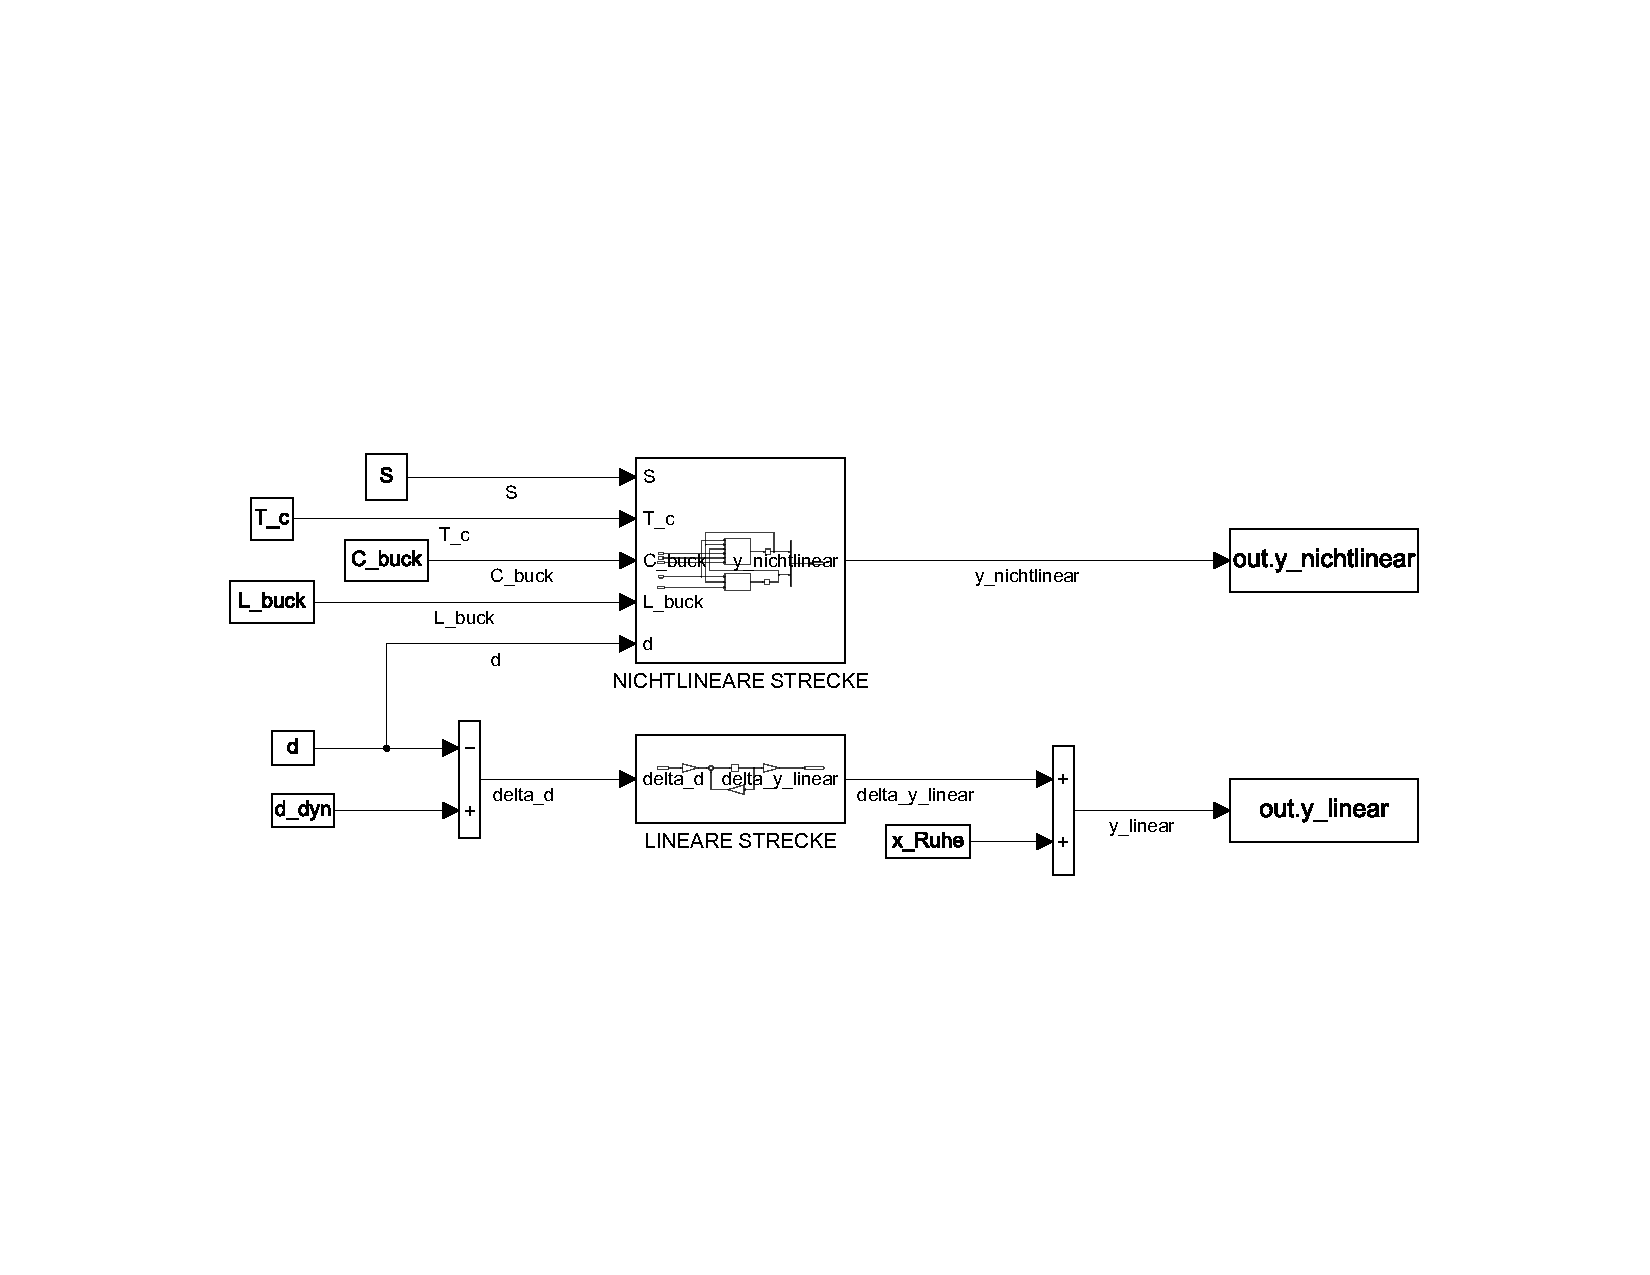
\includegraphics[width=0.65\textwidth]{Bilder/4_vergleich/Vergleich_linear_nichtlinear_Uebersicht.pdf}}
   \caption[Übersicht der Simulationsstruktur]{Übersicht der Simulationsstruktur}
   \label{fig:Bild2}
\end{figure}
\begin{figure}[H]
   \centering
   \fbox{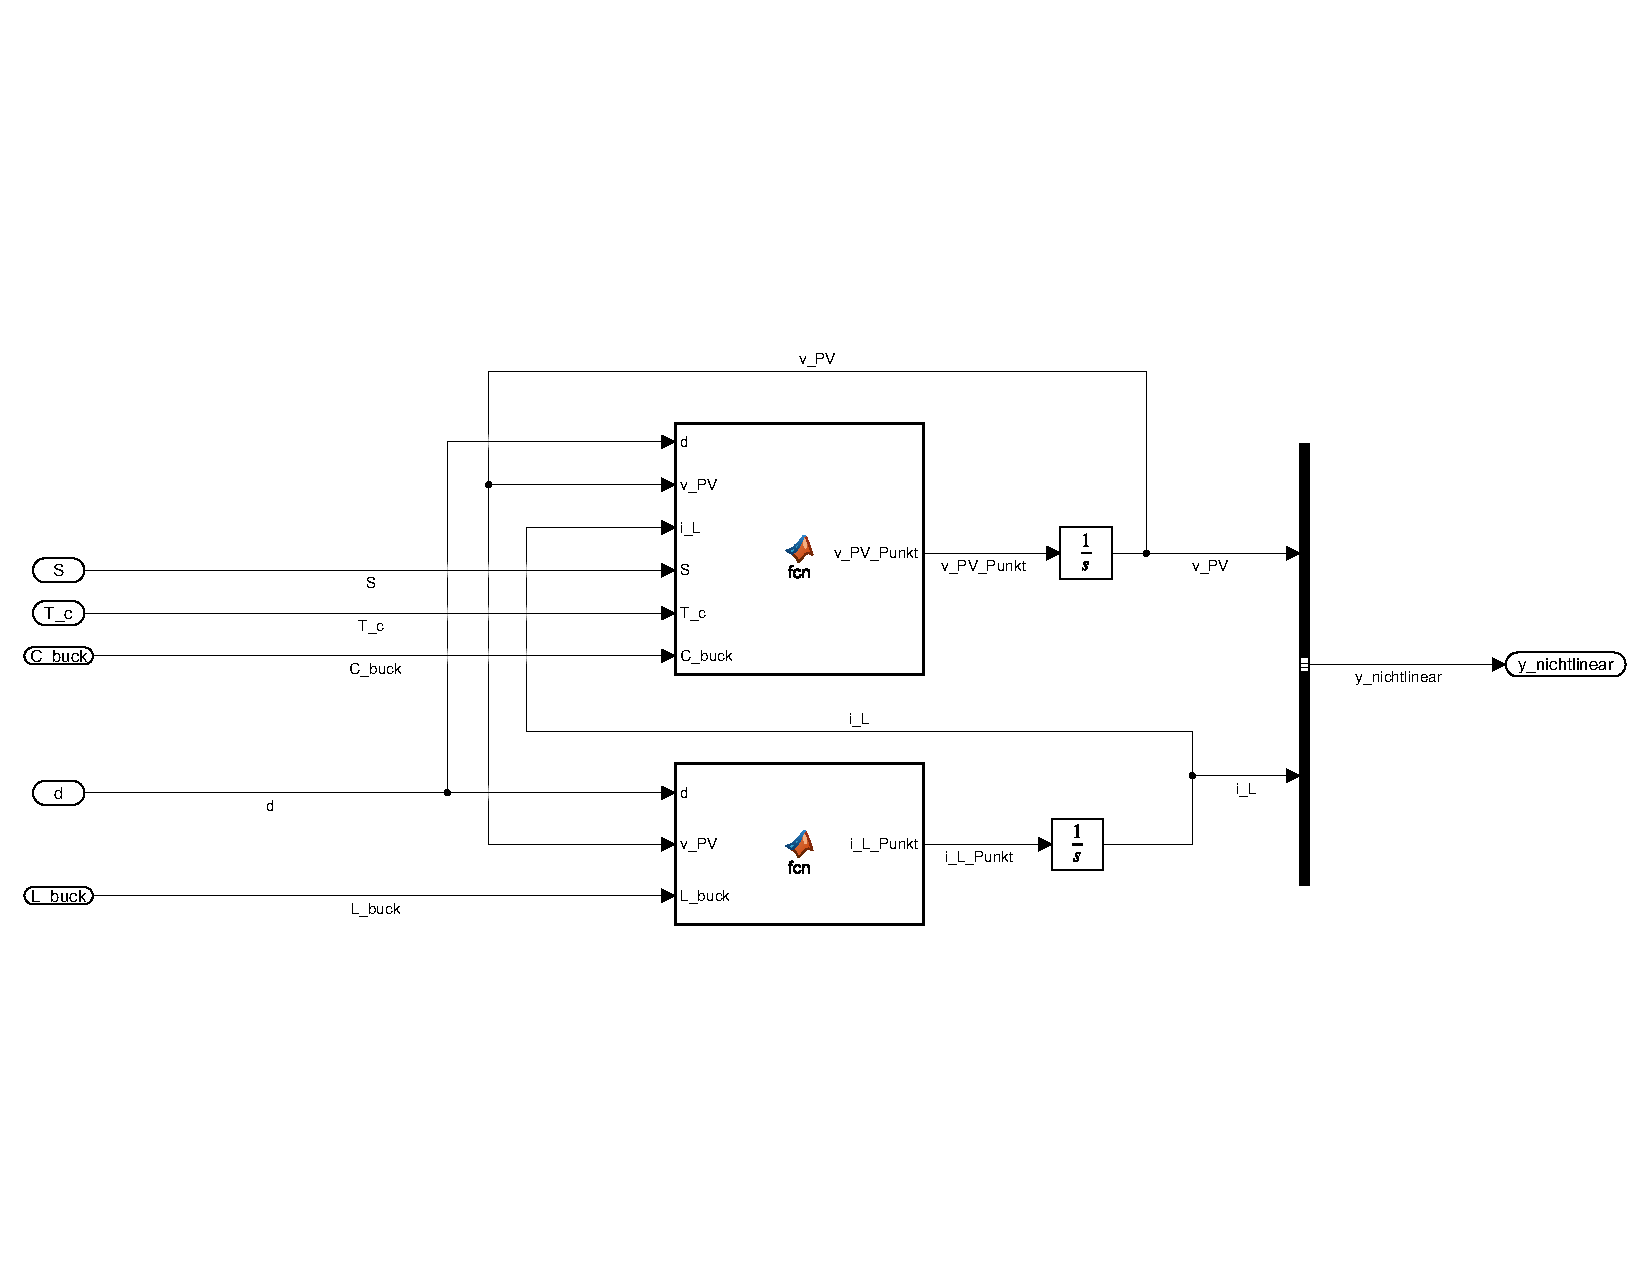
\includegraphics[width=0.65\textwidth]{Bilder/4_vergleich/Vergleich_linear_nichtlinear_Nichtlineare_Strecke.pdf}}
   \caption[Nichtlineare Strecke]{Nichtlineare Strecke}
   \label{fig:Bild3}
\end{figure}
\begin{figure}[H]
   \centering
   \fbox{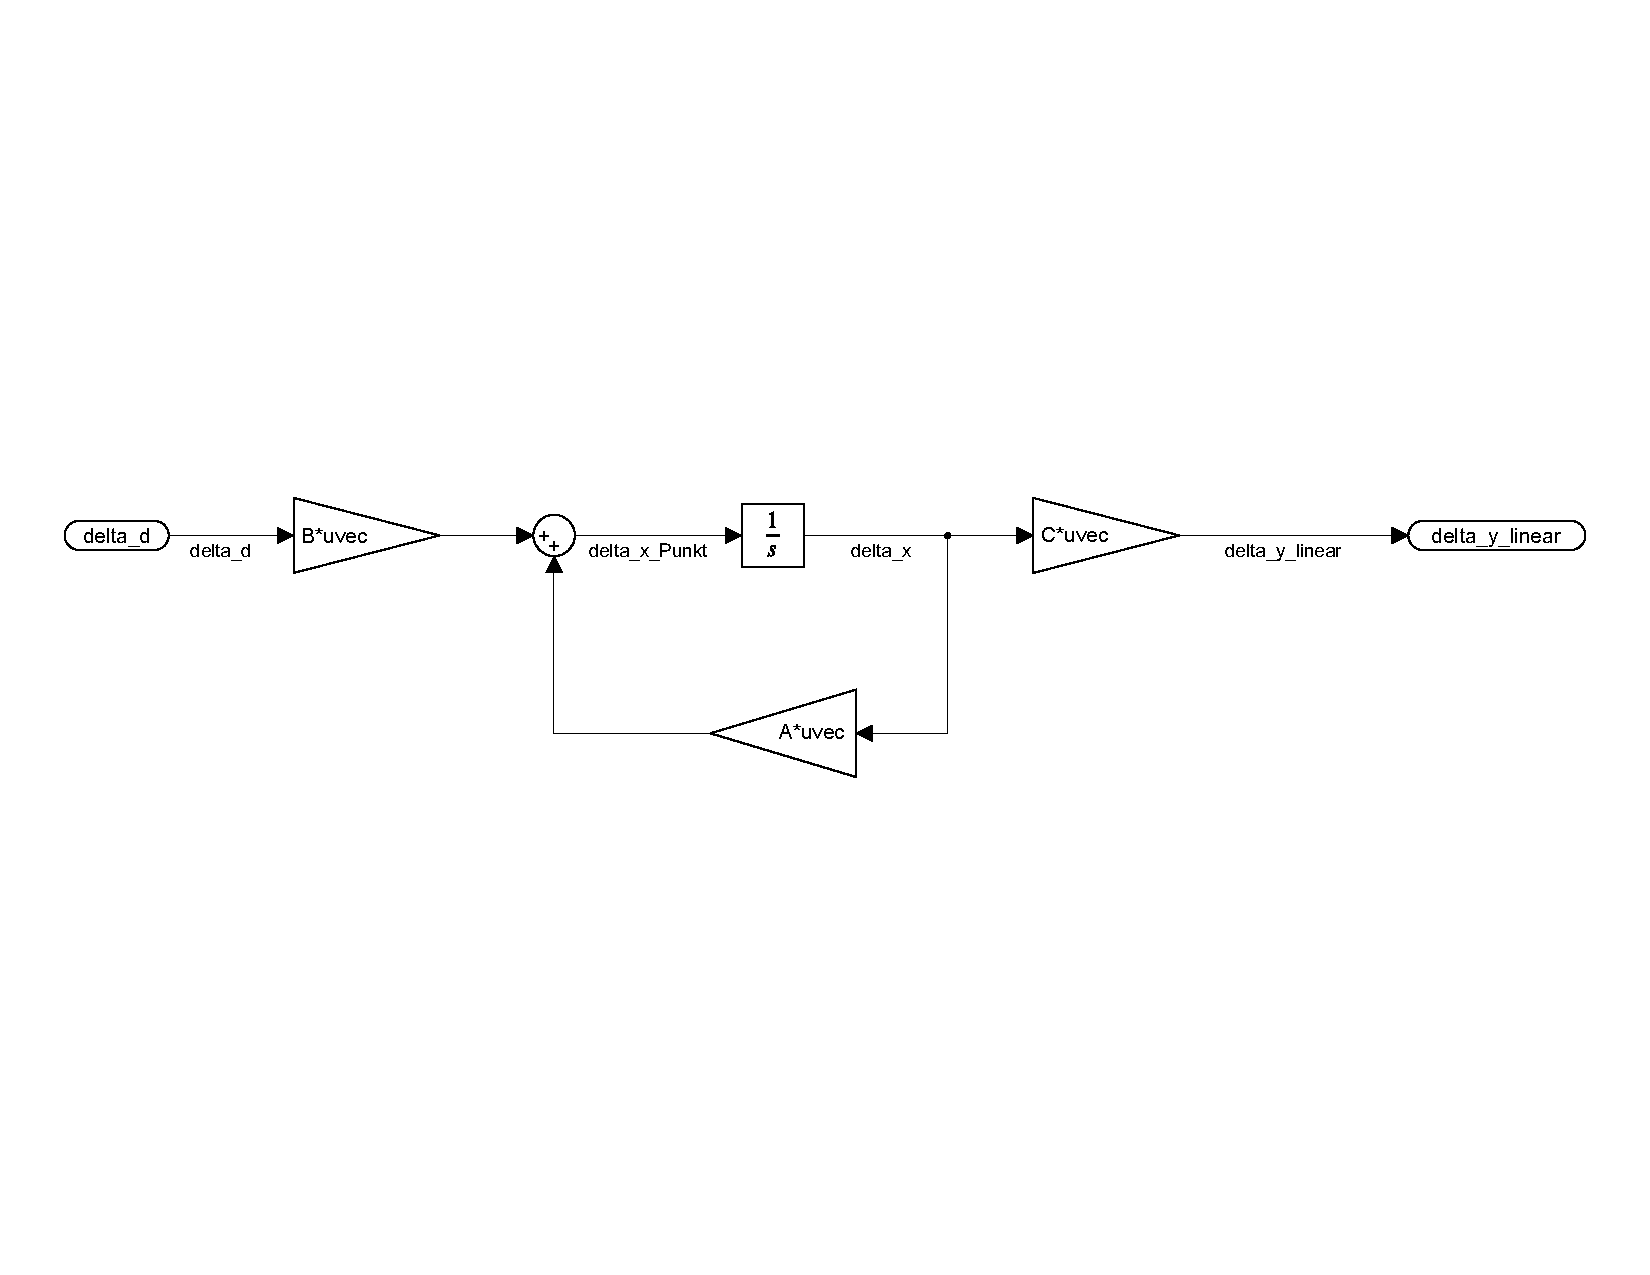
\includegraphics[width=0.65\textwidth]{Bilder/4_vergleich/Vergleich_linear_nichtlinear_Lineare_Strecke.pdf}}
   \caption[Lineare Strecke]{Lineare Strecke}
   \label{fig:Bild4}
\end{figure}

Um das lineare mit dem nichtlinearen Modell zu vergleichen, werden gemäß \autoref{sec:Zustandsraummodell} zu den Zuständen $\Delta \underline{x}$ die Ruhelagen $\underline{x}^*$ aus \autoref{eq:Gleichung12} addiert. Aus der \autoref{fig:Bild5} und \autoref{fig:Bild6} geht hervor, dass die implementierten Systeme für kleine Abweichungen von der Ruhelagen mit steigender Zeit $"t"$ selbiges Verhalten aufweisen.

\begin{figure}[H]
   \centering
   \fbox{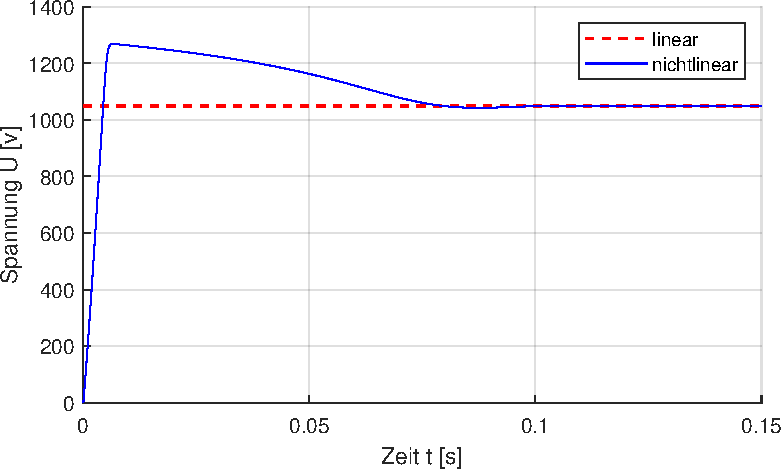
\includegraphics[width=0.7\textwidth]{Bilder/4_vergleich/linear_nichtlinear_vergleich_v_PV.pdf}}
   \caption[Vergleich der Spannungen $v_{\mathrm{PV}}$]{Vergleich der Spannungen $v_{\mathrm{PV}}$ bei -5V Spannungsabweichung zur Ruhelage}
   \label{fig:Bild5}
\end{figure}

\begin{figure}[H]
   \centering
   \fbox{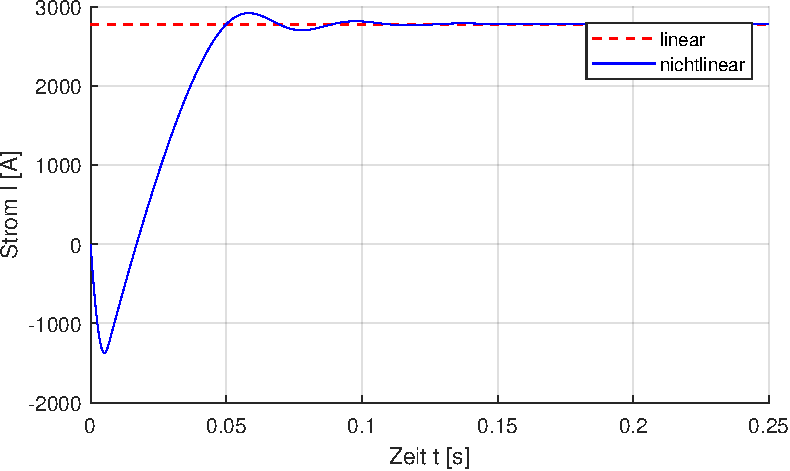
\includegraphics[width=0.7\textwidth]{Bilder/4_vergleich/linear_nichtlinear_vergleich_i_L.pdf}}
   \caption[Vergleich der Ströme $i_{\mathrm{L}}$]{Vergleich der Ströme $i_{\mathrm{L}}$ bei -5V Spannungsabweichung zur Ruhelage}
   \label{fig:Bild6}
\end{figure}


\section{Zustandsreglerentwurf} \label{sec:Zustandsreglerentwurf}

\subsection{Einfache Zustandsrückführung} \label{sec:Einfach}

\subsection{Referenzwertvorsteuerung} \label{sec:Referenzwertvorsteuerung}

\subsection{I-Regelung} \label{sec:Iregler}

\section{Reglervalidierung} \label{sec:Reglervalidierung}

\subsection{Validierung des linearen Modells} \label{sec:Vergleich_linear}

\subsubsection{Zustandsregler mit Ackermann-Formel}

\subsubsection{Zustandsregler mit Vorsteuerung}

\subsubsection{Zustandsregler mit I-Regelung}

\subsubsection{Vergleich des Reglerverhaltens}

\subsection{Validierung des nichtlinearen Modells} \label{sec:Vergleich_nichtlinear}

\subsubsection{Zustandsregler mit Ackermann-Formel}

\subsubsection{Zustandsregler mit Vorsteuerung}

\subsubsection{Zustandsregler mit I-Regelung}

\subsubsection{Vergleich des Reglerverhaltens}


\section{Ausblick} \label{sec:ausblick}

Wie bereits in \autoref{sec:Reglervalidierung} aufgefallen ist, schwingt das System sehr stark bei Reglern mit einfacher Zustandsrückführung und Zustandsreglern mit Referenzwertvorsteuerung. Grund da für ist der Betrag des Imaginärteils der Polstellen, welcher um ein Vielfaches größer ist als der Betrag des Realteils. Um den Imaginärteil zu verkleiner besteht die Möglichkeit die Polregion über LMI's weiter einzuschränken. Der aktuelle Ansatz nutzt lediglich eine Einschränkung über die Vorgabe eines $\alpha$-Wertes, um die Polstellen links einer vorgegebenen Position auf der Real-Achse zu platzieren.\\
Das bisherige LMI könnte über zusätzliche Vorgaben erweitert werden, um die Polregion zu verkleinern \bzw zu optimieren. Dazu wird ein Parameter $r$ für die Auslegung eines Kreisradius um den Koordinatenursprung eingeführt sowie ein $\theta$, um einen Sektor links der Imaginärachse über die Wahl eines Winkels festzulegen. Die sich ergebende Polregion ist in \autoref{fig:Bild27} dargestellt.\\

\begin{figure}[H]
    \centering
    \begin{tikzpicture}[domain=0:0]
        \draw[very thin,color=black] (-0.1,-1.1);                               % Umgebung
        \draw[dashed] (0,-3) arc(270:90:3) -- cycle;                            % Halbkreis
        \draw[-stealth] (0,0) -- (-1.24,2.74);                                  % r-Pfeil
        \node[text width=1cm] at (0, 1.6) {$r$};                                % r
        \draw[dashed] (-0.8,-4) -- (-0.8,4);                                    % alpha-Grenze
        \draw[dashed] (0,0) -- (-3,3);                                          % +theta-Grenze
        \draw[dashed] (0,0) -- (-3,-3);                                         % -theta-Grenze
        \draw[-stealth] (0,-2.5) -- (-0.8,-2.5) node[midway, above] {$\alpha$}; % alpha-Pfeil
        \node[text width=1cm] at (0.6, -0.3) {0};                               % Koordinatenursprung
        \draw[-stealth] (-0.7,0) to [bend left] (-0.5,0.5);                     % theta-Pfeil
        \node[text width=1cm] at (-0.1, 0.2) {$\theta$};                        % theta
        \draw[] (-0.8,-0.8) -- (-0.8,0.8);                                      % Begrenzung rechte Seite des Bereichs
        \node[text width=1cm] at (0, 1.6) {$r$};                                % r
        \begin{scope}
            \clip (-5,-4) rectangle (-0.8,4);
            \draw[pattern={crosshatch}, pattern color=grey] (0,0) -- (-2.12,2.12) arc[start angle=135, delta angle=90,radius=3] -- (0,0); % gefüllter Bereich
        \end{scope}
        \node[text width=3cm] at (-1.2,0.5) {$S(\alpha,r,\theta)$};             % Beschriftung Bereich
        \draw[->] (-4.2,0) -- (2,0) node[right] {$Re$};                         % X-Achse
        \draw[->] (0,-4) -- (0,4) node[above] {$Im$};                           % Y-Achse
    \end{tikzpicture}
    \caption[Polregion bei erweitertem LMI]{Polregion bei Erweiterung des LMI zu $S(\alpha,r,\theta)$}
    \label{fig:Bild27}
\end{figure}

Die Formulierung der erweiterten LMI ist nachfolgend dargestellt:

\begin{align}
    \begin{split}
        \Gamma^1 &= AX + XA^T - BM -M^TB^T + 2\alpha X \\
        \Gamma^2 &=
        \begin{pmatrix}
            (AX + XA^T - BM - M^TB^T)\sin\theta & (AX + XA^T - BM + M^TB^T)\cos\theta \\
            (XA^T - AX - BM - M^TB^T)\cos\theta & (AX + XA^T - BM - M^TB^T)\sin\theta
        \end{pmatrix} \\
        \Gamma^3 &=
        \begin{pmatrix}
            -rX & AX - BM \\
            XA^T - M^TB^T & -rX
        \end{pmatrix}
    \end{split}
\end{align}

% Gainscheduling Regler

%---------Quellen---------------------------------
\newpage
\newcount\Quellennummer
\Quellennummer=1

\renewcommand\refname{Literaturverzeichnis}
\addcontentsline{toc}{section}{Literaturverzeichnis}

\begin{thebibliography}{999}
{\setlength{\emergencystretch}{3cm}%

\bibitem[\the\Quellennummer]{HTWgross}
HTW-Logo auf dem Deckblatt\par
\url{https://de.wikipedia.org/wiki/Datei:Logo_HTW_Berlin.svg} \par
 Stand: 17.08.2018 um 14:49 Uhr

\advance\Quellennummer by 1
 
\bibitem[\the\Quellennummer]{HTWklein}
HTW-Logo in der Kopfzeile\par
\url{http://tonkollektiv-htw.de/} \par
 Stand: 17.08.2018 um 14:53 Uhr

\advance\Quellennummer by 1

\bibitem[\the\Quellennummer]{SkriptSchulte}
Skript Moderne Methoden der Regelungstechnik\par
Prof.\xspace Dr.\xspace -Ing.\xspace Horst Schulte

\advance\Quellennummer by 1

\bibitem[\the\Quellennummer]{LinBrandstaedter}
Anleitung Linearisierung eines zeitinvarianten,\par
nichtlinearen Zustandmodells\par
Prof.\xspace Dr.\xspace -Ing.\xspace Heide Brandstädter

\advance\Quellennummer by 1

\bibitem[\the\Quellennummer]{RegelungBuss}
Regelungs- und Steuerungstechnik: Polstellenverteilung\par
Prof.\xspace Dr.\xspace -Ing.\xspace M. Buss

\advance\Quellennummer by 1

\bibitem[\the\Quellennummer]{BeobachterSchmidt}
Beobachtbarkeit und Beobachter für lineare Kontrollsysteme\par
Judith Schmidt, Universität Bayreuth

\advance\Quellennummer by 1

}
\end{thebibliography}

\end{document}
